\chapter{Конструкторская часть}
\section{Схемы алгоритмов Левенштейна}
Ниже представлены следующие схемы алгоритмов:

рис \ref{png:1} - схема алгоритма итеративного алгоритма Левенштейна с использованием двух строк

рис \ref{png:2} - схема алгоритма рекурсивного алгоритма Левенштейна без кэша

рис \ref{png:3} - схема алгоритма рекурсивного алгоритма Дамерау-Левенштейна с использованием матрицы

рис \ref{png:4} - схема алгоритма итеративного алгоритма Левенштейна с использованием двух строк \\

\section*{Вывод}
На основе теоретических данных, полученных в аналатическом разделе, были построены схемы нужных алгоритмов.

\begin{figure}[pht!]
	\centering{
		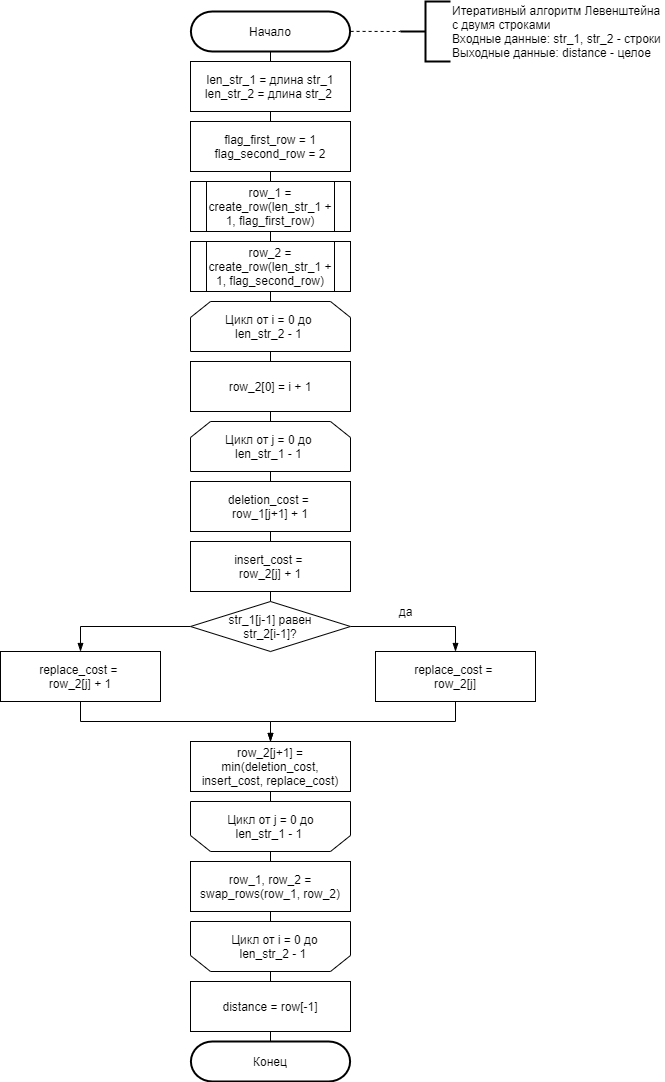
\includegraphics[width=14.6cm]{../../../../../../../msys64/home/Лев/bmstu_sem_5_aa/lab_01/report/diagrams/iterative_two_rows}
		\caption{Сравнение времени работы алгоритмов Левенштейна.}
		\label{png:1}}
\end{figure} 

\begin{figure}[pht!]
	\centering{
		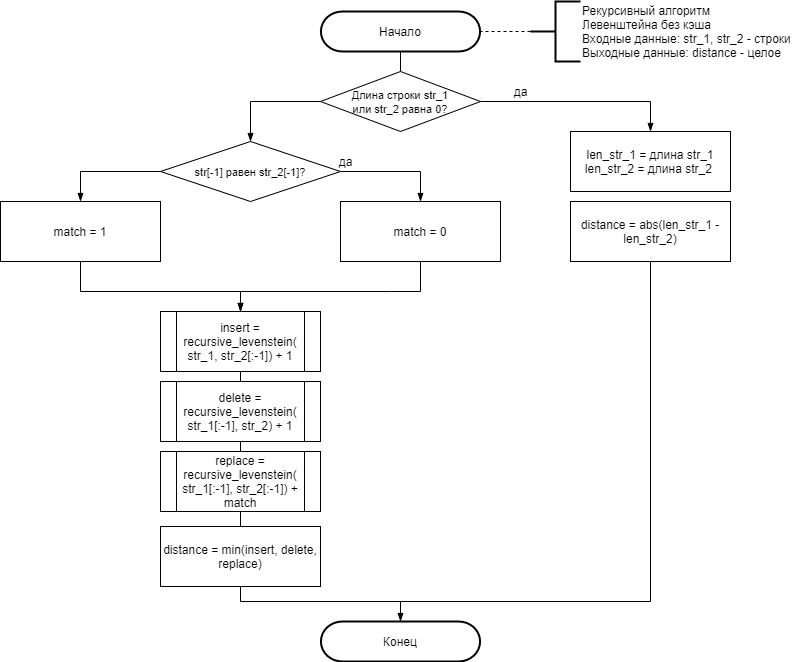
\includegraphics[width=14.6cm]{../../../../../../../msys64/home/Лев/bmstu_sem_5_aa/lab_01/report/diagrams/Рекурсивный Левенштейн без кэша}
		\caption{Сравнение времени работы алгоритмов Левенштейна.}
		\label{png:2}}
\end{figure} 

\begin{figure}[pht!]
	\centering{
		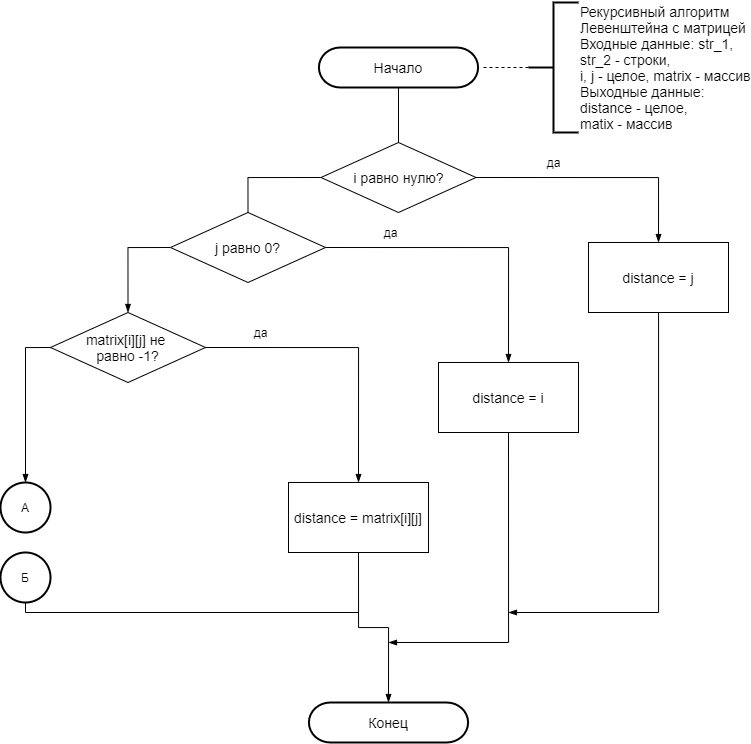
\includegraphics[width=14.6cm]{../../../../../../../msys64/home/Лев/bmstu_sem_5_aa/lab_01/report/diagrams/Рекурсивный Левенштейн с матрицей1}
		\caption{Сравнение времени работы алгоритмов Левенштейна.}
		\label{png:3}}
\end{figure}

\begin{figure}[pht!]
	\centering{
		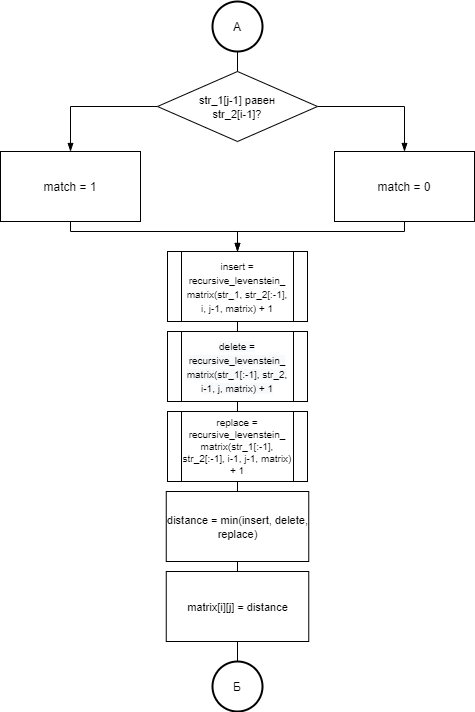
\includegraphics[width=14.6cm]{../../../../../../../msys64/home/Лев/bmstu_sem_5_aa/lab_01/report/diagrams/Рекурсивный Левенштейн с матрицей2}
		\caption{Сравнение времени работы алгоритмов Левенштейна.}
		\label{png:4}}
\end{figure}  
\newpage

\begin{figure}[pht!]
	\centering{
		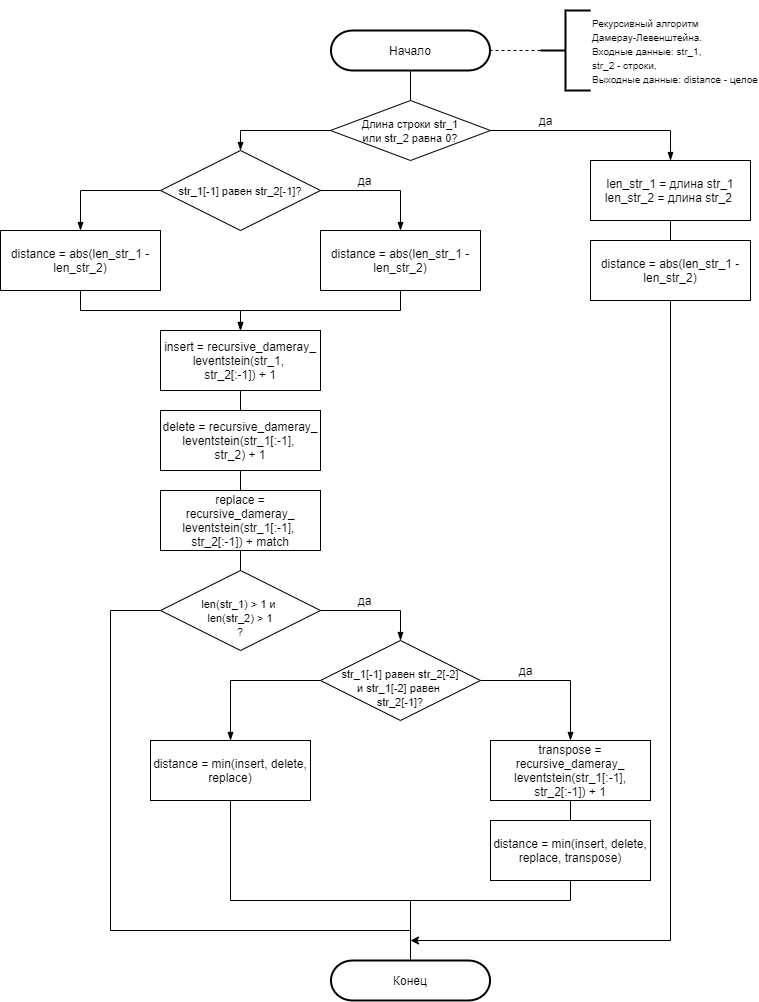
\includegraphics[width=14.6cm]{../../../../../../../msys64/home/Лев/bmstu_sem_5_aa/lab_01/report/diagrams/Рекурсивный Дамерау-Левенштейн}
		\caption{Сравнение времени работы алгоритмов Левенштейна.}
		\label{png:5}}
\end{figure}